\chapter{Literature Review}\label{lreview}
\section{Overview}\label{lroverview}
OkNN problem appears in both AI path planning and Spatial query processing.
Therefore, in this chapter, the literature review includes related works in these two fields.

In section~\ref{lrai}, we introduce two classic pathfinding algorithms:
\textit{Dijkstra} and \textit{A*}, as the historical background.

In section~\ref{lrindex}, we introduce a spatial index \textit{R-tree},
and discuss how it solves traditional kNN problem.

In section~\ref{lrknn}, we focus on existing works on OkNN, two algorithms based on
\textit{Local Visibility Graph} will be discussed. 

In section~\ref{lrnav}, we introduce a very fast point-to-point algorithm in AI path planning
field which shows a new direction to solve OkNN problem.

In section~\ref{lrquery}, we briefly discuss other related spatial queries which can be
improved by our research.

\section{Classic pathfinding}\label{lrai}
The most widely used pathfinding algorithm is \textit{Dijkstra} \cite{dijkstra1959note}. 
The algorithm works on a nonnegative weighted graph, it requires a priority queue and
regards the length of shortest path as key, and it visit vertices in the order
of length of the shortest path until requirements are satisfied, e.g. the target has been found.
When the target is the furthest vertex to the start vertex, \textit{Dijkstra} has to explore the entire
map. Based on such consideration, researchers generalized \textit{Dijkstra} algorithm to
\textit{best-first search} which explores a graph by expanding the most promising node chosen
according to a specified rule.
\textit{A*} \cite{hart1968formal} is known as a famous \textit{best-first search},
it select the path that minimizes:
$$
f(n) = \textit{g-value}(n) + \textit{h-value}(n)
$$
where $n$ is the last node on the path, \textit{g-value} is the length of the shortest path from start to
$n$, \textit{h-value} is an estimation of the shortest path from $n$ to the goal which is
problem-specific. One important property of \textit{h-value} is admissibility, meaning that it never
overestimates the actual cost to the target.
For example, in an Euclidean plane with obstacles, \textit{h-value} can be the Euclidean
distance.

In following sections and the chapter~\ref{proposedalgo}, we will show how \textit{Dijkstra} and
\textit{A*} algorithms be applied on the OkNN problem.

\section{Spatial Index}\label{lrindex}

\subsection{\textit{R-tree}}

\textit{R-tree} has many variations\cite{guttman1984r,beckmann1990r,sellis1987r+,kamel1993hilbert},
they improve efficiency in different aspects,
but they still provide the same functionality,
so we only introduce the classic \textit{R-tree} in this section.

\begin{figure}[htp]
  \centering
  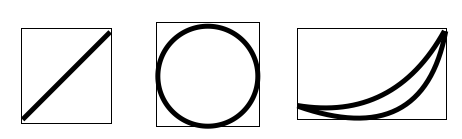
\includegraphics[width=.8\linewidth]{./pic/mbr.png}
  \caption{\small Both segments, circle and irregular shape can be represented by their MBR}
  \label{mbr}
\end{figure}

\textit{R-tree} is a heigh-balanced tree \cite{guttman1984r}, all objects are stored in a leaf
node. In leaf node, if an object is not a point, it would be represented by its \textit{Minimal Bounding
Rectangle} (MBR), figure~\ref{mbr} shows examples of MBR. Each interior node is also
represented by a MBR which contains either leaf nodes or descendant interior nodes.
To guarantee efficiency, each non-root node of \textit{R-tree} can contain at least $m$ entries
and at most $M$ entries, where $m, M$ are specified constant when \textit{R-tree} is built, and
\textit{R-tree}'s root always has two entries. 
Usually, objects retrieval start from the root,
then narrow down to children nodes based on spatial information in their MBRs, and finally
retrieve objects from leaf nodes.
Figure~\ref{rtree} shows how to store and retrieve objects.

\begin{figure}[htp]
  \centering
  \begin{subfigure}{.5\textwidth}
    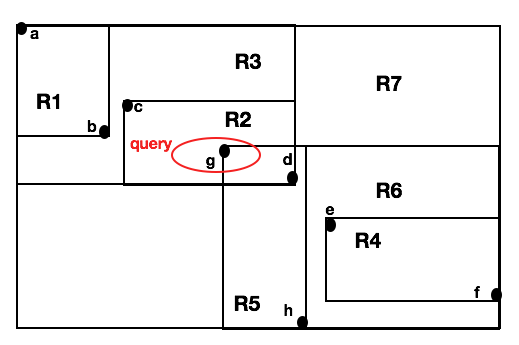
\includegraphics[width=\linewidth]{./pic/hierarchy_mbr.png}
    \caption{Hierachy of MBRs}
    \label{hmbr}
  \end{subfigure}%
  \begin{subfigure}{.5\textwidth}
    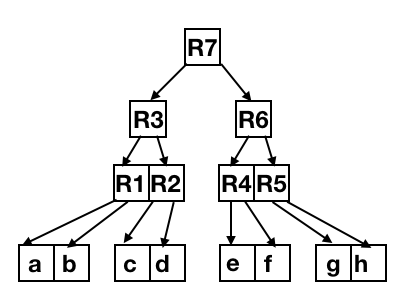
\includegraphics[width=\linewidth]{./pic/rtree.png}
    \caption{Corresponding tree structure}
    \label{tree}
  \end{subfigure}
  \caption{\small $\{a,b,c,d,e,f,g,h\}$ is the object set,
  $R1,R2,R4,R5$ are leaf nodes, $R3,R6$ are interior nodes, and $R7$ is the root.
  The red oval is a range query, starting with $R7$, since $R6$'s MBR overlapped with query
  area, we narrow down to $R6$, then to $R5$, and finally retrieve $g$. Notice that $R3,R2$ also
  overlap with the query, so they will also be visited, but nothing retrieved.
  }
  \label{rtree}
\end{figure}

From the example in figure~\ref{rtree}, we can see that overlapping area will be explored
multiple times in retrieval progress, which duplicated efforts.
Thus, some variants use strict non-overlapping interior node (e.g.
$R^+\textit{-tree}$\cite{sellis1987r+}), and non-overlapping \textit{R-tree} is a wide topic in
the spatial index field which beyond the scope of this thesis.

\subsection{Nearest Neighbor Query}
In the \textit{R-tree}, all nodes are organized by their spatial information,
so that the nearest neighbor of a point can be retrieved by exploring tree nodes in some order.
To introduce the algorithm, we need to discuss two metrics: given query point $q$ and the MBR of a tree node
\begin{itemize}
  \item \textit{\textbf{mindist}} is the minimal distance from $q$ to the MBR, it estimates the
    distance from $q$ to inside object, so this metric is the priority of the tree node;
  \item \textit{\textbf{minmaxdist}} is the upper bound of the NN distance of any object inside
    the MBR, if the $mindist$ of any MBR large than this value, then such MBR cannot contains
    the nearest object, so this metric is for pruning.
\end{itemize}
The algorithm starts with root node and proceeds down the tree. When it visits a leaf node,
current nearest neighbor will be updated;
When it visits a non-leaf node, the children of such node is sorted by \textit{mindist}, and pruned by
\textit{minmaxdist}, then algorithm does \textit{depth-first-search} on ordered and pruned children nodes;
when algorithm finished, the updated nearest neighbor is the answer, and it can be easily
generalized to finding kNN by changes below:
\begin{itemize}
  \item  Tracking k current nearest neighbors, instead of one.
  \item  The pruning is according to the current k-th nearest neighbor.
\end{itemize}

This kind of algorithm is called \textit{branch-and-bound} traversal, which has been well
studied and widely used in other artificial intelligence areas\cite{sellis1987r+},
and most existing NN queries are based on it with different ordering and pruning strategies,
more details are in \cite{roussopoulos1995nearest,cheung1998enhanced}.

\section{Obstacle k-Nearest Neighbor}\label{lrknn}

In OkNN problem, the metric is obstacle distance,
so all existing OkNN algorithms are actually Obstacle Distance Computation (ODC).
In following subsections, we introduce these ODC algorithms and show how to apply them on OkNN.

\subsection{In-main-memory OkNN}
Solving obstacle path problems in-main-memory has been well studied \cite{de2000computational},
these works need to compute visibility graph which any pair of co-visible vertices has an edge,
figure~\ref{vg} shows an example.
\begin{figure}[htp]
  \centering
  \begin{tikzpicture}[scale=0.8]
  %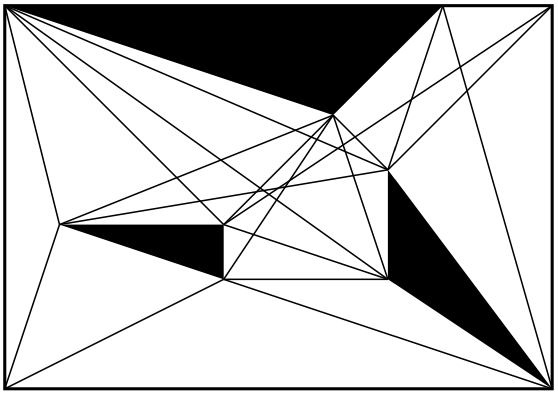
\includegraphics[width=.6\linewidth]{pic/vg.png}
    %\coordinate (a) at (2, 6); 
\coordinate (a) at (0, 7);
\coordinate (b) at (8, 7); 
\coordinate (c) at (6, 5); 
\coordinate (d) at (1, 3);
\coordinate (e) at (4, 3);
\coordinate (f) at (4, 2);
\coordinate (g) at (7, 4);
\coordinate (h) at (7, 2);
%\coordinate (i) at (9, 0);
\coordinate (i) at (10, 0);
\coordinate (j) at (5, 2);
\coordinate (k) at (0, 7);
\coordinate (l) at (0, 0);
\coordinate (m) at (10, 0);
\coordinate (n) at (10, 7);
\coordinate (q) at (3, 4);
\coordinate (Q) at (3, 4);
\coordinate (t) at (9, 3);
\coordinate (o) at (7.5, 5.5);

\newcommand{\nodelabel}[2] {
    \node[fill,circle,scale=0.25,label=#2:$#1$,color=red] at (#1) {$#1$};
}

\newcommand{\medge}[2]{
    \draw[gray,thick] (#1)--(#2);
}

\newcommand{\vgedge}[2]{
    \draw[black,thick] (#1)--(#2);
}

\newcommand{\drawVs}{
    %\nodelabel{a}{above}
    \nodelabel{b}{below}
    \nodelabel{c}{below}
    
    %\nodelabel{d}{left}
    \nodelabel{e}{right}
    \nodelabel{f}{below}
    
    \nodelabel{g}{above}
    \nodelabel{h}{below}
    %\nodelabel{i}{below}
}

\newcommand{\drawmeshs}{
    \medge{a}{k},\medge{a}{d},\medge{a}{b},\medge{a}{c}
    \medge{b}{c},
    \medge{c}{g}
    \medge{d}{f},\medge{d}{l},\medge{d}{e}
    \medge{l}{f}
    \medge{e}{c},\medge{e}{f}
    \medge{f}{h}
    \medge{g}{h},\medge{g}{b}
    \medge{h}{i}
}

\newcommand{\drawobstacles}{
    \fill[black] (a)--(b)--(c)--cycle;
    \fill[black] (g)--(h)--(i)--cycle;
    \fill[black] (d)--(e)--(f)--cycle;
}

\newcommand{\drawstart} {
    % \fill[blue] (q) circle[radius=.5ex];
    % \node[above] at (q) {$q$};
    \node[fill,circle,scale=0.25,label=above:$q$,color=blue] at (q) {$q$};

}

\newcommand{\drawend}{
    \fill[blue] (t) circle[radius=.5ex];
    \node[above] at (t) {$t$};
}

\newcommand{\drawboundary}{
    \draw[black, ultra thick] (k)--(n)--(m)--(l)--cycle;
}

\newcommand{\showvisible} {
    \fill[lightgray] (c)--(e)--(d)--(a);
    \nodelabel{e}{right}
    \nodelabel{c}{below}
    \drawstart;
}

\newcommand{\stepa} {
    \fill[lightgray] (c)--(e)--(d)--(a);
    \fill[lightgray] (c)--(g)--(h)--(f)--(e);
    \draw[black, thin] (q)--(g);
    \draw[green, very thick] (e)--(c);
    \drawstart
    \drawVs
}

\newcommand{\stepb} {
    \fill[lightgray] (c)--(e)--(d)--(a);
    \fill[lightgray] (c)--(g)--(h)--(f)--(e);
    \fill[lightgray] (c)--(g)--(b);
    \draw[black, thin] (q)--(g);
    \draw[green, very thick] (e)--(c);
    \draw[black, thin] (g)--(t);
    \draw[black, thin] (q)--(g);
    \draw[green, very thick] (g)--(c);
    \draw[green, very thick] (g)--(b);
    \drawstart
    \drawend
    \drawVs
}

\newcommand{\polyanyaexpand}{
    \draw[black,very thin, dashed] (q)--($(q)!5cm!(e)$);
    \draw[black,very thin, dashed] (q)--($(q)!5cm!(c)$);
    \draw[orange!50, line width=3pt] (j)--(h);
    \draw[orange!50, line width=3pt] (h)--(g);
    \draw[orange!50, line width=3pt] (g)--(c);
    \draw[cyan, line width=3pt] (e)--(f);
    \draw[cyan, line width=3pt] (f)--(j);
}

\newcommand{\drawVG}{
    \vgedge{a}{d},\vgedge{a}{e},\vgedge{a}{g},\vgedge{a}{h}
    \vgedge{b}{g},\vgedge{b}{m}
    \vgedge{c}{d},\vgedge{c}{e},\vgedge{c}{g},\vgedge{c}{f},\vgedge{c}{h}
    \vgedge{d}{l},\vgedge{d}{g}
    \vgedge{e}{h},\vgedge{e}{n}
    \vgedge{f}{l},\vgedge{f}{h},\vgedge{f}{m}
    \vgedge{g}{n}
}
\newcommand{\drawmap}{
    \drawboundary
    \drawobstacles
    \drawmeshs
    \drawVs
    \drawstart
    \drawend
}

\newcommand{\intervalexpansion}{
    \drawboundary
    \drawobstacles
    \drawmeshs
    {\draw[green!50, line width=3pt, dashed] (e)--(d);}
    {\draw[green!50, line width=3pt, dashed] (d)--(a);}
    {\draw[green!50, line width=3pt, dashed] (a)--(c);}
    {\draw[green!50, line width=3pt, dashed] (e)--(c);}
    {\draw[green!50, line width=3pt, dashed] (d)--(l);}
    {\draw[green!50, line width=3pt, dashed] (e)--(f);}
    {\draw[green!50, line width=3pt, dashed] (f)--(j);}
    {\draw[green!50, line width=3pt, dashed] (j)--(h);}
    {\draw[green!50, line width=3pt, dashed] (g)--(h);}
    {\draw[green!50, line width=3pt, dashed] (c)--(g);}
    {\draw[green!50, line width=3pt, dashed] (g)--(b);}
    {\draw[black, line width=3pt] (q)--(g);}
    {\draw[black, line width=3pt] (g)--(t);}
    \drawstart
    \drawend 
    \drawVs
}

    \drawboundary
    \drawobstacles
    \drawVG
  \end{tikzpicture}
  \caption{\small The rectangle is the boundary of the map, black polygons are obstacles and all
  black lines are edges in the visibility graph.}
  \label{vg}
\end{figure}

Since all edges of the shortest path belong to visibility graph \cite{lozano1979algorithm},
once precomputed it and include visible edges from query point, we can run shortest path
algorithm (e.g. \textit{Dijkstra}) to find k-nearest neighbor.
However, precomputing visibility graph(VG) is costly:
even the best algorithm \cite{ghosh1991output} has
$O(m + nlogn)$ runtime, where $n$ is the number of vertexes and $m$ is the number of edges,
and in practice, $m$ can reach to $O(n^2)$.
In spatial database scenario, $n$ can be more than $10,000$, so in-main-memory approach is not
suitable for spatial database scenario.

\subsection{Local Visibility Graph}

Since building global VG is infeasible, researchers in spatial database field
are motivated to design an algorithm that only considers query related area.

In 2004, Zhang proposed the \textit{Local Visibility Graph} (LVG) algorithm\cite{zhang2004spatial}
to compute obstacle distance.
Assume obstacles are stored in \textit{R-tree},
given query point $q$, and a target $t$, the algorithm runs in
following steps:
\begin{enumerate}
    \item It starts with a small VG centered on $q$ with radius $r=d_e(q, t)$ (figure~\ref{edbt1});
    \item Then compute shortest path on the current VG (figure~\ref{edbt2});
    \item Enlarge the circle to current obstacle distance $r=d_o(q,t)$, update the VG
      incrementally (figure~\ref{edbt2}) and recompute the shortest path (figure~\ref{edbt4});
    \item Repeat the previous step until $r>=d_o(q, t)$.
\end{enumerate}

\begin{figure*}[!h]
  \begin{subfigure}{\linewidth}
    \centering
    \begin{subfigure}{.45\linewidth}
      \centering
      \begin{tikzpicture}[line cap=round,line join=round,>=triangle 45,x=1.0cm,y=1.0cm]
\definecolor{aqaqaq}{rgb}{0.6274509803921569,0.6274509803921569,0.6274509803921569}
\definecolor{qqqqff}{rgb}{0.,0.,1.}
\clip(1.6,0.47) rectangle (6.28,5.17);
\draw [line width=1.2pt,color=aqaqaq,fill=aqaqaq,fill opacity=0.3499999940395355] (3.9400050555577426,2.815716717828029) circle (1.cm);
\fill[line width=1.2pt,fill=black,fill opacity=1.0] (1.7619906352802,3.2064019550048823) -- (1.760948257574785,2.966272798087264) -- (5.9009925693289444,3.0440732742639014) -- (6.065992717197827,3.275305213897039) -- cycle;
\fill[line width=1.2pt,fill=black,fill opacity=1.0] (2.7838752248591803,3.776985670170509) -- (2.5711486339617498,3.69319853872332) -- (2.5711499019374466,3.389901746844879) -- (2.8995061535758593,3.4158740479215886) -- cycle;
\draw [line width=1.2pt] (1.7619906352802,3.2064019550048823)-- (1.760948257574785,2.966272798087264);
\draw [line width=1.2pt] (1.760948257574785,2.966272798087264)-- (5.9009925693289444,3.0440732742639014);
\draw [line width=1.2pt] (5.9009925693289444,3.0440732742639014)-- (6.065992717197827,3.275305213897039);
\draw [line width=1.2pt] (6.065992717197827,3.275305213897039)-- (1.7619906352802,3.2064019550048823);
\draw [line width=1.2pt] (2.7838752248591803,3.776985670170509)-- (2.5711486339617498,3.69319853872332);
\draw [line width=1.2pt] (2.5711486339617498,3.69319853872332)-- (2.5711499019374466,3.389901746844879);
\draw [line width=1.2pt] (2.5711499019374466,3.389901746844879)-- (2.8995061535758593,3.4158740479215886);
\draw [line width=1.2pt] (2.8995061535758593,3.4158740479215886)-- (2.7838752248591803,3.776985670170509);
\draw [line width=1.2pt] (1.760948257574785,2.9662727980872643)-- (1.7619906352802033,3.206401955004883);
\begin{scriptsize}
\draw [fill=qqqqff] (3.9400050555577426,2.815716717828029) circle (2.5pt);
\draw[color=qqqqff] (4.380260269409033,2.521369672358508) node {$q$};
\draw [fill=qqqqff] (3.8997931043534932,3.8149078902171505) circle (2.5pt);
\draw[color=qqqqff] (4.079705546011023,4.182329985873814) node {$t$};
\end{scriptsize}
\end{tikzpicture}
      \caption{
        \small 
        the long rectangle obstacle in the\\
        circle is retrieved and included in vg.
      }
      \label{edbt1}
    \end{subfigure}%
    \begin{subfigure}{.45\linewidth}
      \centering
      \begin{tikzpicture}[line cap=round,line join=round,>=triangle 45,x=1.0cm,y=1.0cm]
\definecolor{aqaqaq}{rgb}{0.6274509803921569,0.6274509803921569,0.6274509803921569}
\definecolor{qqqqff}{rgb}{0.,0.,1.}
\clip(1.6,0.47) rectangle (6.28,5.17);
\draw [line width=1.2pt,color=aqaqaq,fill=aqaqaq,fill opacity=0.3499999940395355] (3.9400050555577426,2.815716717828029) circle (1.cm);
\fill[line width=1.2pt,fill=black,fill opacity=1.0] (1.7619906352802,3.2064019550048823) -- (1.760948257574785,2.966272798087264) -- (5.9009925693289444,3.0440732742639014) -- (6.065992717197827,3.275305213897039) -- cycle;
\fill[line width=1.2pt,fill=black,fill opacity=1.0] (2.7838752248591803,3.776985670170509) -- (2.5711486339617498,3.69319853872332) -- (2.5711499019374466,3.389901746844879) -- (2.8995061535758593,3.4158740479215886) -- cycle;
\draw [line width=1.2pt] (1.7619906352802,3.2064019550048823)-- (1.760948257574785,2.966272798087264);
\draw [line width=1.2pt] (1.760948257574785,2.966272798087264)-- (5.9009925693289444,3.0440732742639014);
\draw [line width=1.2pt] (5.9009925693289444,3.0440732742639014)-- (6.065992717197827,3.275305213897039);
\draw [line width=1.2pt] (6.065992717197827,3.275305213897039)-- (1.7619906352802,3.2064019550048823);
\draw [line width=1.2pt] (2.7838752248591803,3.776985670170509)-- (2.5711486339617498,3.69319853872332);
\draw [line width=1.2pt] (2.5711486339617498,3.69319853872332)-- (2.5711499019374466,3.389901746844879);
\draw [line width=1.2pt] (2.5711499019374466,3.389901746844879)-- (2.8995061535758593,3.4158740479215886);
\draw [line width=1.2pt] (2.8995061535758593,3.4158740479215886)-- (2.7838752248591803,3.776985670170509);
\draw [line width=1.2pt] (3.9400050555577426,2.815716717828029)-- (1.760948257574785,2.9662727980872643);
\draw [line width=1.2pt] (1.760948257574785,2.9662727980872643)-- (1.7619906352802033,3.206401955004883);
\draw [line width=1.2pt] (1.7619906352802033,3.206401955004883)-- (3.8997931043534932,3.8149078902171505);
\begin{scriptsize}
\draw [fill=qqqqff] (3.9400050555577426,2.815716717828029) circle (2.5pt);
\draw[color=qqqqff] (4.380260269409033,2.521369672358508) node {$q$};
\draw [fill=qqqqff] (3.8997931043534932,3.8149078902171505) circle (2.5pt);
\draw[color=qqqqff] (4.079705546011023,4.182329985873814) node {$t$};
\end{scriptsize}
\end{tikzpicture}
      \caption{
        \small current shortest path may be blocked by some obstacles outside
      }
      \label{edbt2}
    \end{subfigure}
  \end{subfigure}\par\medskip
  \begin{subfigure}{\linewidth}
    \centering
    \begin{subfigure}{.45\linewidth}
      \centering
      \begin{tikzpicture}[line cap=round,line join=round,>=triangle 45,x=1.0cm,y=1.0cm]
\definecolor{aqaqaq}{rgb}{0.6274509803921569,0.6274509803921569,0.6274509803921569}
\definecolor{qqqqff}{rgb}{0.,0.,1.}
\clip(1.6,0.47) rectangle (6.28,5.17);
\draw [line width=1.2pt,color=aqaqaq,fill=aqaqaq,fill opacity=0.3499999940395355] (3.9400050555577426,2.815716717828029) circle (1.cm);
\fill[line width=1.2pt,fill=black,fill opacity=1.0] (1.7619906352802,3.2064019550048823) -- (1.760948257574785,2.966272798087264) -- (5.9009925693289444,3.0440732742639014) -- (6.065992717197827,3.275305213897039) -- cycle;
\fill[line width=1.2pt,fill=black,fill opacity=1.0] (2.7838752248591803,3.776985670170509) -- (2.5711486339617498,3.69319853872332) -- (2.5711499019374466,3.389901746844879) -- (2.8995061535758593,3.4158740479215886) -- cycle;
\draw [line width=1.2pt,color=aqaqaq,fill=aqaqaq,fill opacity=0.25] (3.9400050555577426,2.815716717828029) circle (2.3cm);
\draw [line width=1.2pt] (1.7619906352802,3.2064019550048823)-- (1.760948257574785,2.966272798087264);
\draw [line width=1.2pt] (1.760948257574785,2.966272798087264)-- (5.9009925693289444,3.0440732742639014);
\draw [line width=1.2pt] (5.9009925693289444,3.0440732742639014)-- (6.065992717197827,3.275305213897039);
\draw [line width=1.2pt] (6.065992717197827,3.275305213897039)-- (1.7619906352802,3.2064019550048823);
\draw [line width=1.2pt] (2.7838752248591803,3.776985670170509)-- (2.5711486339617498,3.69319853872332);
\draw [line width=1.2pt] (2.5711486339617498,3.69319853872332)-- (2.5711499019374466,3.389901746844879);
\draw [line width=1.2pt] (2.5711499019374466,3.389901746844879)-- (2.8995061535758593,3.4158740479215886);
\draw [line width=1.2pt] (2.8995061535758593,3.4158740479215886)-- (2.7838752248591803,3.776985670170509);
\draw [line width=1.2pt] (3.9400050555577426,2.815716717828029)-- (1.760948257574785,2.9662727980872643);
\draw [line width=1.2pt] (1.760948257574785,2.9662727980872643)-- (1.7619906352802033,3.206401955004883);
\draw [line width=1.2pt] (1.7619906352802033,3.206401955004883)-- (3.8997931043534932,3.8149078902171505);
\begin{scriptsize}
\draw [fill=qqqqff] (3.9400050555577426,2.815716717828029) circle (2.5pt);
\draw[color=qqqqff] (4.380260269409033,2.521369672358508) node {$q$};
\draw [fill=qqqqff] (3.8997931043534932,3.8149078902171505) circle (2.5pt);
\draw[color=qqqqff] (4.079705546011023,4.182329985873814) node {$t$};
\end{scriptsize}
\end{tikzpicture}
      \caption{
        \small enlarges the circle and updates the vg
      }
      \label{edbt3}
    \end{subfigure}%
    \begin{subfigure}{.45\linewidth}
      \centering
      \begin{tikzpicture}[line cap=round,line join=round,>=triangle 45,x=1.0cm,y=1.0cm]
\definecolor{aqaqaq}{rgb}{0.6274509803921569,0.6274509803921569,0.6274509803921569}
\definecolor{qqqqff}{rgb}{0.,0.,1.}
\clip(1.6,0.47) rectangle (6.28,5.17);
\draw [line width=1.2pt,color=aqaqaq,fill=aqaqaq,fill opacity=0.3499999940395355] (3.9400050555577426,2.815716717828029) circle (1.cm);
\fill[line width=1.2pt,fill=black,fill opacity=1.0] (1.7619906352802,3.2064019550048823) -- (1.760948257574785,2.966272798087264) -- (5.9009925693289444,3.0440732742639014) -- (6.065992717197827,3.275305213897039) -- cycle;
\fill[line width=1.2pt,fill=black,fill opacity=1.0] (2.7838752248591803,3.776985670170509) -- (2.5711486339617498,3.69319853872332) -- (2.5711499019374466,3.389901746844879) -- (2.8995061535758593,3.4158740479215886) -- cycle;
\draw [line width=1.2pt,color=aqaqaq,fill=aqaqaq,fill opacity=0.25] (3.9400050555577426,2.815716717828029) circle (2.3cm);
\draw [line width=1.2pt] (1.7619906352802,3.2064019550048823)-- (1.760948257574785,2.966272798087264);
\draw [line width=1.2pt] (1.760948257574785,2.966272798087264)-- (5.9009925693289444,3.0440732742639014);
\draw [line width=1.2pt] (5.9009925693289444,3.0440732742639014)-- (6.065992717197827,3.275305213897039);
\draw [line width=1.2pt] (6.065992717197827,3.275305213897039)-- (1.7619906352802,3.2064019550048823);
\draw [line width=1.2pt] (2.7838752248591803,3.776985670170509)-- (2.5711486339617498,3.69319853872332);
\draw [line width=1.2pt] (2.5711486339617498,3.69319853872332)-- (2.5711499019374466,3.389901746844879);
\draw [line width=1.2pt] (2.5711499019374466,3.389901746844879)-- (2.8995061535758593,3.4158740479215886);
\draw [line width=1.2pt] (2.8995061535758593,3.4158740479215886)-- (2.7838752248591803,3.776985670170509);
\draw [line width=1.2pt] (3.9400050555577426,2.815716717828029)-- (1.760948257574785,2.9662727980872643);
\draw [line width=1.2pt] (1.760948257574785,2.9662727980872643)-- (1.7619906352802033,3.206401955004883);
\draw [line width=1.2pt] (1.7619906352802033,3.206401955004883)-- (2.5711499019374506,3.389901746844879);
\draw [line width=1.2pt] (2.8995061535758624,3.415874047921588)-- (3.8997931043534932,3.8149078902171505);
\begin{scriptsize}
\draw [fill=qqqqff] (3.9400050555577426,2.815716717828029) circle (2.5pt);
\draw[color=qqqqff] (4.30746415449908,2.57569402093485) node {$q$};
\draw [fill=qqqqff] (3.8997931043534932,3.8149078902171505) circle (2.5pt);
\draw[color=qqqqff] (4.042501567145657,4.1257251569523605) node {$t$};
\end{scriptsize}
\end{tikzpicture}
      \caption{
        \small recomputes the shortest path  
      }
      \label{edbt4}
    \end{subfigure}
  \end{subfigure}
  \caption{\small LVG algorithm}
\end{figure*}

When algorithm finish, since $r>=d_o(q, t)$, it guarantees that no obstacle on the current shortest
path, and thus proving the correctness. This algorithm can be extended to multi-target
scenario to solve OkNN problem:
\begin{itemize}
  \item Initially, $t$ is the \textit{k-th} nearest neighbor in Euclidean space, so that it
    guarantees that the VG always contains at least $k$ targets;
  \item Terminate when $r$  not less than the current \textit{k-th} nearest distance;
\end{itemize}

\subsection{Fast filter}

There's another similar work proposed by Xia\cite{xia2004fast},
the difference is, instead of considering obstacles in a circle area,
it only retrieves obstacles on the current shortest path,
updates the LVG and recomputes the shortest path.
Since fewer obstacles are involved in VG,
the algorithm is called \textit{Fast Filter}.
Figure~\ref{xia} shows an example.
\begin{figure*}[!h]
  \centering
  \begin{subfigure}{.45\linewidth}
    \centering
    \begin{tikzpicture}[line cap=round,line join=round,>=triangle 45,x=0.6cm,y=0.6cm]
\definecolor{yqyqyq}{rgb}{0.5019607843137255,0.5019607843137255,0.5019607843137255}
\definecolor{wqwqwq}{rgb}{0.3764705882352941,0.3764705882352941,0.3764705882352941}
\definecolor{ududff}{rgb}{0.30196078431372547,0.30196078431372547,1.}
\definecolor{cqcqcq}{rgb}{0.7529411764705882,0.7529411764705882,0.7529411764705882}
\draw [color=cqcqcq,, xstep=4.0cm,ystep=4.0cm] (-2.,-0.7) grid (5.5,6.);
\clip(-2.,-0.7) rectangle (5.5,6.);
\fill[line width=2.pt,fill=black,fill opacity=1.0] (3.,4.) -- (3.,-0.5) -- (4.,-0.5) -- (4.,4.) -- cycle;
\fill[line width=2.pt,fill=black,fill opacity=1.0] (2.,6.) -- (1.958260850221742,2.42739675673013) -- (-2.036562862356449,2.42739675673013) -- (-2.,6.) -- cycle;
\draw [line width=2.pt] (3.,4.)-- (4.,4.);
\draw [line width=2.pt,color=wqwqwq] (4.,4.)-- (5.,2.);
\draw [line width=2.pt] (3.,-0.5)-- (4.,-0.5);
\draw [line width=2.pt,color=wqwqwq] (-1.,2.)-- (3.,4.);
\draw [line width=2.pt,dash pattern=on 7pt off 7pt,color=yqyqyq] (-1.,2.)-- (5.,2.);
\begin{scriptsize}
\draw [fill=ududff] (-1.,2.) circle (2.5pt);
\draw[color=ududff] (-1.3610221733554015,1.519358046860102) node {$q$};
\draw [fill=ududff] (5.,2.) circle (2.5pt);
\draw[color=ududff] (5.163642125127989,2.4314078950351963) node {$t$};
\draw [fill=ududff] (3.,4.) circle (2.5pt);
\draw [fill=ududff] (3.,-0.5) circle (2.5pt);
\draw [fill=ududff] (4.,-0.5) circle (2.5pt);
\draw [fill=ududff] (4.,4.) circle (2.5pt);
\end{scriptsize}
\end{tikzpicture}

    \caption{}
    \label{xia0}
  \end{subfigure}%
  \begin{subfigure}{.45\linewidth}
    \centering
    \begin{tikzpicture}[line cap=round,line join=round,>=triangle 45,x=.6cm,y=.6cm]
\definecolor{yqyqyq}{rgb}{0.5019607843137255,0.5019607843137255,0.5019607843137255}
\definecolor{wqwqwq}{rgb}{0.3764705882352941,0.3764705882352941,0.3764705882352941}
\definecolor{ududff}{rgb}{0.30196078431372547,0.30196078431372547,1.}
\definecolor{cqcqcq}{rgb}{0.7529411764705882,0.7529411764705882,0.7529411764705882}
\draw [color=cqcqcq,, xstep=4.0cm,ystep=4.0cm] (-2.,-0.7) grid (5.5,6.);
\clip(-2.,-0.7) rectangle (5.5,6.);
\fill[line width=2.pt,fill=black,fill opacity=1.0] (3.,4.) -- (3.,-0.5) -- (4.,-0.5) -- (4.,4.) -- cycle;
\fill[line width=2.pt,fill=black,fill opacity=1.0] (2.,6.) -- (1.958260850221742,2.42739675673013) -- (-2.036562862356449,2.42739675673013) -- (-2.,6.) -- cycle;
\draw [line width=2.pt] (3.,4.)-- (4.,4.);
\draw [line width=2.pt,dash pattern=on 3pt off 3pt,color=wqwqwq] (4.,4.)-- (5.,2.);
\draw [line width=2.pt,color=wqwqwq] (-1.,2.)-- (3.,-0.5);
\draw [line width=2.pt] (3.,-0.5)-- (4.,-0.5);
\draw [line width=2.pt,color=wqwqwq] (4.,-0.5)-- (5.,2.);
\draw [line width=2.pt,dash pattern=on 3pt off 3pt,color=wqwqwq] (-1.,2.)-- (3.,4.);
\draw [line width=2.pt,dash pattern=on 7pt off 7pt,color=yqyqyq] (-1.,2.)-- (5.,2.);
\begin{scriptsize}
\draw [fill=ududff] (-1.,2.) circle (2.5pt);
\draw[color=ududff] (-1.3607039979330486,1.5168391580998075) node {$q$};
\draw [fill=ududff] (5.,2.) circle (2.5pt);
\draw[color=ududff] (5.172498007716814,2.426820866029606) node {$t$};
\draw [fill=ududff] (3.,4.) circle (2.5pt);
\draw [fill=ududff] (3.,-0.5) circle (2.5pt);
\draw [fill=ududff] (4.,-0.5) circle (2.5pt);
\draw [fill=ududff] (4.,4.) circle (2.5pt);
\end{scriptsize}
\end{tikzpicture}

    \caption{}
    \label{xia1}
  \end{subfigure}
  \caption{
    \small Black polygons are obstacles,
    $q$ is query point, $t$ is the target.
    Initially, the VG only contains
    the rectangle obstacle between the $qt$,
    and the corresponding shortest path is computed (fig~\ref{xia0}).
    Then retrieves the square
    obstacle on the current path,
    updates VG and recomputes the shortest path (fig~\ref{xia1}).
  }
  \label{xia}
\end{figure*}

To solve OkNN, we need following changes:
\begin{itemize}
  \item initially compute obstacle distance for k nearest neighbors, and store results in
    \textit{max-heap} with size $k$;
  \item keep retrieving next NN and compute the obstacle distance $d_o$;
  \item when $d_o$ not large than the top value of heap, pop top and insert the current $d_o$;
  \item terminate when the Euclidean distance to current NN is large than the Obstacle distance
    on top of the heap;
\end{itemize}
\subsection{Discussion}
When search space is large (e.g. target is far from the query point), \textit{fast
filter}\cite{xia2004fast} is
more efficient because it only considers obstacles that might on the path, meanwhile
\textit{LVG}\cite{zhang2004spatial} will build visibility graph for a large area, which is slow. 
In a multi-target scenario, when $k$ is large, \textit{LVG}\cite{zhang2004spatial} is more efficient because
\textit{Dijkstra} is a natural single-source algorithm, meanwhile, each time \textit{fast
filter}\cite{xia2004fast} can
only compute the path for a single target, so that it duplicates effort for common prefixes of $k$
targets.

Both \textit{LVG}\cite{zhang2004spatial} and \textit{Fast filter}\cite{xia2004fast} are simple to understand,
provide optimality guarantees and the promise of fast performance. Such advantages make them
attractive to researchers and, despite more than a decade since their introduction,
they continue to appear as ingredients in a variety of kNN studies from the literature; e.g.
\cite{gao2011efficient,gao2016reverse}.
However, these visibility graph based algorithms also suffer from a number of notable
disadvantages including:
\begin{enumerate}[label=(\roman*)]
  \item costly online visibility checks;
  \item an incremental construction process that has up to quadratic space and time complexity for the worst case;
  \item duplicated efforts are unavoidable, since the graph is discarded each time the query point changes.
\end{enumerate}

\section{Pathfinding on Navigation Mesh}\label{lrnav}

\subsection{Historical background}
Because of the limitation of VG, \textit{Navigation Mesh} comes to our sight.
Ronald first proposed this concept in 1986\cite{ronald1986pathfinding}, then it is applied on
robotics and game pathfinding.

Navigation mesh divides traversable space into convex polygons, the convexity of mesh
guarantees that all insides points are co-visible so that it not needs visibility checking,
Figure~\ref{nav} shows an example.
Compare to VG (fig~\ref{vg}), it can be generated by\textit{Constrained Delaunay
Triangulation}\cite{chew1989constrained} in $O(nlogn)$ times,
so that it is feasible to preprocess the entire map.
Additionally, adding or removing obstacles only needs to modify a few numbers of mesh polygons,
which is very flexible. It seems like a perfect framework for OkNN,
the only problem is that how to compute obstacle distance on it.

\begin{figure}[htp]
  \centering
  \begin{tikzpicture}[scale=0.8]
    %\coordinate (a) at (2, 6); 
\coordinate (a) at (0, 7);
\coordinate (b) at (8, 7); 
\coordinate (c) at (6, 5); 
\coordinate (d) at (1, 3);
\coordinate (e) at (4, 3);
\coordinate (f) at (4, 2);
\coordinate (g) at (7, 4);
\coordinate (h) at (7, 2);
%\coordinate (i) at (9, 0);
\coordinate (i) at (10, 0);
\coordinate (j) at (5, 2);
\coordinate (k) at (0, 7);
\coordinate (l) at (0, 0);
\coordinate (m) at (10, 0);
\coordinate (n) at (10, 7);
\coordinate (q) at (3, 4);
\coordinate (Q) at (3, 4);
\coordinate (t) at (9, 3);
\coordinate (o) at (7.5, 5.5);

\newcommand{\nodelabel}[2] {
    \node[fill,circle,scale=0.25,label=#2:$#1$,color=red] at (#1) {$#1$};
}

\newcommand{\medge}[2]{
    \draw[gray,thick] (#1)--(#2);
}

\newcommand{\vgedge}[2]{
    \draw[black,thick] (#1)--(#2);
}

\newcommand{\drawVs}{
    %\nodelabel{a}{above}
    \nodelabel{b}{below}
    \nodelabel{c}{below}
    
    %\nodelabel{d}{left}
    \nodelabel{e}{right}
    \nodelabel{f}{below}
    
    \nodelabel{g}{above}
    \nodelabel{h}{below}
    %\nodelabel{i}{below}
}

\newcommand{\drawmeshs}{
    \medge{a}{k},\medge{a}{d},\medge{a}{b},\medge{a}{c}
    \medge{b}{c},
    \medge{c}{g}
    \medge{d}{f},\medge{d}{l},\medge{d}{e}
    \medge{l}{f}
    \medge{e}{c},\medge{e}{f}
    \medge{f}{h}
    \medge{g}{h},\medge{g}{b}
    \medge{h}{i}
}

\newcommand{\drawobstacles}{
    \fill[black] (a)--(b)--(c)--cycle;
    \fill[black] (g)--(h)--(i)--cycle;
    \fill[black] (d)--(e)--(f)--cycle;
}

\newcommand{\drawstart} {
    % \fill[blue] (q) circle[radius=.5ex];
    % \node[above] at (q) {$q$};
    \node[fill,circle,scale=0.25,label=above:$q$,color=blue] at (q) {$q$};

}

\newcommand{\drawend}{
    \fill[blue] (t) circle[radius=.5ex];
    \node[above] at (t) {$t$};
}

\newcommand{\drawboundary}{
    \draw[black, ultra thick] (k)--(n)--(m)--(l)--cycle;
}

\newcommand{\showvisible} {
    \fill[lightgray] (c)--(e)--(d)--(a);
    \nodelabel{e}{right}
    \nodelabel{c}{below}
    \drawstart;
}

\newcommand{\stepa} {
    \fill[lightgray] (c)--(e)--(d)--(a);
    \fill[lightgray] (c)--(g)--(h)--(f)--(e);
    \draw[black, thin] (q)--(g);
    \draw[green, very thick] (e)--(c);
    \drawstart
    \drawVs
}

\newcommand{\stepb} {
    \fill[lightgray] (c)--(e)--(d)--(a);
    \fill[lightgray] (c)--(g)--(h)--(f)--(e);
    \fill[lightgray] (c)--(g)--(b);
    \draw[black, thin] (q)--(g);
    \draw[green, very thick] (e)--(c);
    \draw[black, thin] (g)--(t);
    \draw[black, thin] (q)--(g);
    \draw[green, very thick] (g)--(c);
    \draw[green, very thick] (g)--(b);
    \drawstart
    \drawend
    \drawVs
}

\newcommand{\polyanyaexpand}{
    \draw[black,very thin, dashed] (q)--($(q)!5cm!(e)$);
    \draw[black,very thin, dashed] (q)--($(q)!5cm!(c)$);
    \draw[orange!50, line width=3pt] (j)--(h);
    \draw[orange!50, line width=3pt] (h)--(g);
    \draw[orange!50, line width=3pt] (g)--(c);
    \draw[cyan, line width=3pt] (e)--(f);
    \draw[cyan, line width=3pt] (f)--(j);
}

\newcommand{\drawVG}{
    \vgedge{a}{d},\vgedge{a}{e},\vgedge{a}{g},\vgedge{a}{h}
    \vgedge{b}{g},\vgedge{b}{m}
    \vgedge{c}{d},\vgedge{c}{e},\vgedge{c}{g},\vgedge{c}{f},\vgedge{c}{h}
    \vgedge{d}{l},\vgedge{d}{g}
    \vgedge{e}{h},\vgedge{e}{n}
    \vgedge{f}{l},\vgedge{f}{h},\vgedge{f}{m}
    \vgedge{g}{n}
}
\newcommand{\drawmap}{
    \drawboundary
    \drawobstacles
    \drawmeshs
    \drawVs
    \drawstart
    \drawend
}

\newcommand{\intervalexpansion}{
    \drawboundary
    \drawobstacles
    \drawmeshs
    {\draw[green!50, line width=3pt, dashed] (e)--(d);}
    {\draw[green!50, line width=3pt, dashed] (d)--(a);}
    {\draw[green!50, line width=3pt, dashed] (a)--(c);}
    {\draw[green!50, line width=3pt, dashed] (e)--(c);}
    {\draw[green!50, line width=3pt, dashed] (d)--(l);}
    {\draw[green!50, line width=3pt, dashed] (e)--(f);}
    {\draw[green!50, line width=3pt, dashed] (f)--(j);}
    {\draw[green!50, line width=3pt, dashed] (j)--(h);}
    {\draw[green!50, line width=3pt, dashed] (g)--(h);}
    {\draw[green!50, line width=3pt, dashed] (c)--(g);}
    {\draw[green!50, line width=3pt, dashed] (g)--(b);}
    {\draw[black, line width=3pt] (q)--(g);}
    {\draw[black, line width=3pt] (g)--(t);}
    \drawstart
    \drawend 
    \drawVs
}

    {
    \drawboundary
    \drawobstacles
    \drawmeshs
    }
  \end{tikzpicture}
  \caption{\small Navigation Mesh: The rectangle is the boundary of the map, black polygons are
  obstacles, gray lines are edges of mesh polygons.}
  \label{nav}
\end{figure}

Previous pathfinding algorithms on navigation mesh are not suitable for spatial query
processing, and thus it's not attractive to researchers in this fields.
Three widely used algorithms are:
\begin{itemize}
\item Channel Search \cite{kallmann2005path}: first find an abstract path from start to target
    composed of polygons, then refine the abstract path to a sequence of concrete points. This
    algorithm only generate an approximately shortest path, the lack of optimality makes it not
    suitable for OkNN query.
  \item TA* \cite{demyen2006efficient}: similar to Channel Search, but it can repeat the search
    process until finding an optimal shortest path. The repeating is time-consuming, so it is not
    suitable for query processing.
  \item TRA* \cite{demyen2006efficient}: similar to TA*, but TRA* can utilize preprocessing to
    speed up pathfinding. The problem is that the precomputed information will be invalid when
    the environment change, so it is not suitable for database scenario.
\end{itemize}

However, this fact has been changed by a recent work called
\textit{Polyanya}\cite{cuicompromise}. It is a fast, optimal and flexible pathfinding algorithm
which is perfect for query processing in spatial database.

\subsection{Polyanya}\label{lrpoly}
\textit{Polyanya} can be seen as an instance of \textit{A*}: it performs a best-first search
using an admissible heuristic function to prioritize nodes. The mechanical details are however
quite different, there are three key components:
\begin{itemize}
\item \textbf{Search Nodes}: Conventional  search algorithms proceed from one traversable point
  to the next. \textit{Polyanya}, by comparison, searches from one \textit{edge} of the
  navigation mesh to another. In this model, search nodes are tuples $(I, r)$ where each
  $I=[a,b]$ is a contiguous interval of points and $r$ is a distinguished point called the
  \textit{root}. Nodes are constructed such that each point $p \in I$ is visible from $r$.
  Meanwhile, $r$ itself corresponds to the last turning point on the path: from $q$ to any $p
  \in I$. Figure~\ref{snode} shows an example.

  \begin{figure}[htb]
    \centering
     %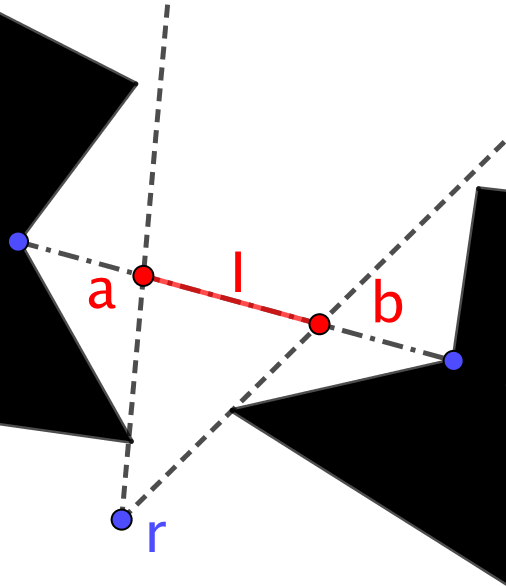
\includegraphics[width=.5\linewidth]{pic/snode.png}
    \begin{tikzpicture}[line cap=round,line join=round,>=triangle 45,x=1.5cm,y=1.5cm]
\definecolor{ffqqqq}{rgb}{1.,0.,0.}
\definecolor{ududff}{rgb}{0.30196078431372547,0.30196078431372547,1.}
\clip(-0.8,-1.6) rectangle (4.5,1.9);
\fill[line width=2.pt,fill=black,fill opacity=1.0] (1.0568852561643571,1.7160911807341181) -- (-0.05223307140302057,0.7078017920365031) -- (0.8888370247147546,-0.23326830408127103) -- (-0.8588645823611135,-0.09882971892158902) -- (-0.8084501129262327,1.2623609558201914) -- cycle;
\fill[line width=2.pt,fill=black,fill opacity=1.0] (1.823359787139688,-0.3207843311089217) -- (3.2477722134398506,0.38019461763527085) -- (3.1845504618814697,1.6117703305615074) -- (4.915447245812395,-0.5392470319934045) -- cycle;
\draw [thick] (-0.05223307140302057,0.7078017920365031)-- (3.2477722134398506,0.38019461763527085);
\draw [dash pattern=on 2pt off 2pt,domain=-0.8:1.0362283883022219] plot(\x,{(-1.0239487358475874--1.1906912514220491*\x)/-0.1473913635874673});
\draw [dash pattern=on 2pt off 2pt,domain=1.0362283883022219:4.5] plot(\x,{(-2.2639847616004545--1.1031752243943984*\x)/0.7871313988374662});
\draw [line width=2.pt,color=ffqqqq] (2.3846562728722773,0.4658802302519392)-- (0.7826045650521551,0.6249235007746435);
\begin{scriptsize}
\draw [fill=ududff] (-0.05223307140302057,0.7078017920365031) circle (2.5pt);
\draw [fill=ududff] (3.2477722134398506,0.38019461763527085) circle (2.5pt);
\draw [fill=ududff] (1.0362283883022219,-1.4239595555033202) circle (2.5pt);
\draw[color=ududff] (0.7743350405885554,-1.3148373272892926) node {\large $r$};
\draw [fill=ffqqqq] (2.3846562728722773,0.4658802302519392) circle (2.0pt);
\draw[color=ffqqqq] (2.767634409298129,0.6348131501346688) node {\large $b$};
\draw [fill=ffqqqq] (0.7826045650521551,0.6249235007746435) circle (2.0pt);
\draw[color=ffqqqq] (0.45424317116074064,0.8967064978483352) node {\large $a$};
\draw[color=ffqqqq] (1.6473128663007772,0.9112561282768722) node {\large $I$};
\end{scriptsize}
\end{tikzpicture}

    \caption{\small Search nodes in Polyanya. Notice that the interval $I = [a, b]$ is
    a contiguous subset of points drawn from an edge of the navigation mesh.
    The corresponding root point, $r$, is either the query point itself 
    or the vertex of an obstacle. Taken together they form the search node $(I, r)$.}
    \label{snode}
  \end{figure}

\item \textbf{Successors}: Successor nodes $(I', r')$ are generated by "pushing" the current
  interval $I$ away from its root $r$ and throught the interior of an adjacent and traversable
  polygon. A successor is said to be \textit{obervable} if each point $p' \in I'$ is visible
  from $r$. The successor node in this case is formed by the tuple $(I',r)$. By contrast, a
  successor is said to be \textit{non-observable} if the \textit{taut} (i.e. locally optimal)
  path from $r$ to each $p' \in I'$ must pass through one of the endpoints of current interval
  $I=[a,b]$. The successor node in this case is formed by the tuple $(I', r')$ with $r'$ as
  one of the points $a$ or $b$. Figure~\ref{suc} shows an example.
 
  Note that the target point is inserted in the open list as a special case
  (observable or non-observable) successor whenever the search reaches its 
  containing polygon.  The interval of this successor contains only the target.
  \begin{figure}[ht]
    \centering
    \begin{tikzpicture}
      %\coordinate (a) at (2, 6); 
\coordinate (a) at (0, 7);
\coordinate (b) at (8, 7); 
\coordinate (c) at (6, 5); 
\coordinate (d) at (1, 3);
\coordinate (e) at (4, 3);
\coordinate (f) at (4, 2);
\coordinate (g) at (7, 4);
\coordinate (h) at (7, 2);
%\coordinate (i) at (9, 0);
\coordinate (i) at (10, 0);
\coordinate (j) at (5, 2);
\coordinate (k) at (0, 7);
\coordinate (l) at (0, 0);
\coordinate (m) at (10, 0);
\coordinate (n) at (10, 7);
\coordinate (q) at (3, 4);
\coordinate (Q) at (3, 4);
\coordinate (t) at (9, 3);
\coordinate (o) at (7.5, 5.5);

\newcommand{\nodelabel}[2] {
    \node[fill,circle,scale=0.25,label=#2:$#1$,color=red] at (#1) {$#1$};
}

\newcommand{\medge}[2]{
    \draw[gray,thick] (#1)--(#2);
}

\newcommand{\vgedge}[2]{
    \draw[black,thick] (#1)--(#2);
}

\newcommand{\drawVs}{
    %\nodelabel{a}{above}
    \nodelabel{b}{below}
    \nodelabel{c}{below}
    
    %\nodelabel{d}{left}
    \nodelabel{e}{right}
    \nodelabel{f}{below}
    
    \nodelabel{g}{above}
    \nodelabel{h}{below}
    %\nodelabel{i}{below}
}

\newcommand{\drawmeshs}{
    \medge{a}{k},\medge{a}{d},\medge{a}{b},\medge{a}{c}
    \medge{b}{c},
    \medge{c}{g}
    \medge{d}{f},\medge{d}{l},\medge{d}{e}
    \medge{l}{f}
    \medge{e}{c},\medge{e}{f}
    \medge{f}{h}
    \medge{g}{h},\medge{g}{b}
    \medge{h}{i}
}

\newcommand{\drawobstacles}{
    \fill[black] (a)--(b)--(c)--cycle;
    \fill[black] (g)--(h)--(i)--cycle;
    \fill[black] (d)--(e)--(f)--cycle;
}

\newcommand{\drawstart} {
    % \fill[blue] (q) circle[radius=.5ex];
    % \node[above] at (q) {$q$};
    \node[fill,circle,scale=0.25,label=above:$q$,color=blue] at (q) {$q$};

}

\newcommand{\drawend}{
    \fill[blue] (t) circle[radius=.5ex];
    \node[above] at (t) {$t$};
}

\newcommand{\drawboundary}{
    \draw[black, ultra thick] (k)--(n)--(m)--(l)--cycle;
}

\newcommand{\showvisible} {
    \fill[lightgray] (c)--(e)--(d)--(a);
    \nodelabel{e}{right}
    \nodelabel{c}{below}
    \drawstart;
}

\newcommand{\stepa} {
    \fill[lightgray] (c)--(e)--(d)--(a);
    \fill[lightgray] (c)--(g)--(h)--(f)--(e);
    \draw[black, thin] (q)--(g);
    \draw[green, very thick] (e)--(c);
    \drawstart
    \drawVs
}

\newcommand{\stepb} {
    \fill[lightgray] (c)--(e)--(d)--(a);
    \fill[lightgray] (c)--(g)--(h)--(f)--(e);
    \fill[lightgray] (c)--(g)--(b);
    \draw[black, thin] (q)--(g);
    \draw[green, very thick] (e)--(c);
    \draw[black, thin] (g)--(t);
    \draw[black, thin] (q)--(g);
    \draw[green, very thick] (g)--(c);
    \draw[green, very thick] (g)--(b);
    \drawstart
    \drawend
    \drawVs
}

\newcommand{\polyanyaexpand}{
    \draw[black,very thin, dashed] (q)--($(q)!5cm!(e)$);
    \draw[black,very thin, dashed] (q)--($(q)!5cm!(c)$);
    \draw[orange!50, line width=3pt] (j)--(h);
    \draw[orange!50, line width=3pt] (h)--(g);
    \draw[orange!50, line width=3pt] (g)--(c);
    \draw[cyan, line width=3pt] (e)--(f);
    \draw[cyan, line width=3pt] (f)--(j);
}

\newcommand{\drawVG}{
    \vgedge{a}{d},\vgedge{a}{e},\vgedge{a}{g},\vgedge{a}{h}
    \vgedge{b}{g},\vgedge{b}{m}
    \vgedge{c}{d},\vgedge{c}{e},\vgedge{c}{g},\vgedge{c}{f},\vgedge{c}{h}
    \vgedge{d}{l},\vgedge{d}{g}
    \vgedge{e}{h},\vgedge{e}{n}
    \vgedge{f}{l},\vgedge{f}{h},\vgedge{f}{m}
    \vgedge{g}{n}
}
\newcommand{\drawmap}{
    \drawboundary
    \drawobstacles
    \drawmeshs
    \drawVs
    \drawstart
    \drawend
}

\newcommand{\intervalexpansion}{
    \drawboundary
    \drawobstacles
    \drawmeshs
    {\draw[green!50, line width=3pt, dashed] (e)--(d);}
    {\draw[green!50, line width=3pt, dashed] (d)--(a);}
    {\draw[green!50, line width=3pt, dashed] (a)--(c);}
    {\draw[green!50, line width=3pt, dashed] (e)--(c);}
    {\draw[green!50, line width=3pt, dashed] (d)--(l);}
    {\draw[green!50, line width=3pt, dashed] (e)--(f);}
    {\draw[green!50, line width=3pt, dashed] (f)--(j);}
    {\draw[green!50, line width=3pt, dashed] (j)--(h);}
    {\draw[green!50, line width=3pt, dashed] (g)--(h);}
    {\draw[green!50, line width=3pt, dashed] (c)--(g);}
    {\draw[green!50, line width=3pt, dashed] (g)--(b);}
    {\draw[black, line width=3pt] (q)--(g);}
    {\draw[black, line width=3pt] (g)--(t);}
    \drawstart
    \drawend 
    \drawVs
}

      \drawmap
      \fill[lightgray] (e)--(f)--(h)--(g)--(c);
      \draw[black,very thin, dashed] (q)--($(q)!6cm!(e)$);
      \draw[black,very thin, dashed] (q)--($(q)!6cm!(c)$);
      \draw[green, line width=3pt] (j)--(h);
      \draw[green, line width=3pt] (h)--(g);
      \draw[green, line width=3pt] (g)--(c);
      \draw[green, line width=5pt, dashed] (c)--(e);
      \draw[orange!50, line width=3pt] (j)--(h);
      \draw[orange!50, line width=3pt] (h)--(g);
      \draw[orange!50, line width=3pt] (g)--(c);
      \draw[cyan, line width=3pt] (e)--(f);
      \draw[cyan, line width=3pt] (f)--(j);
      \drawVs     
      \nodelabel{j}{below}
    \end{tikzpicture}
    %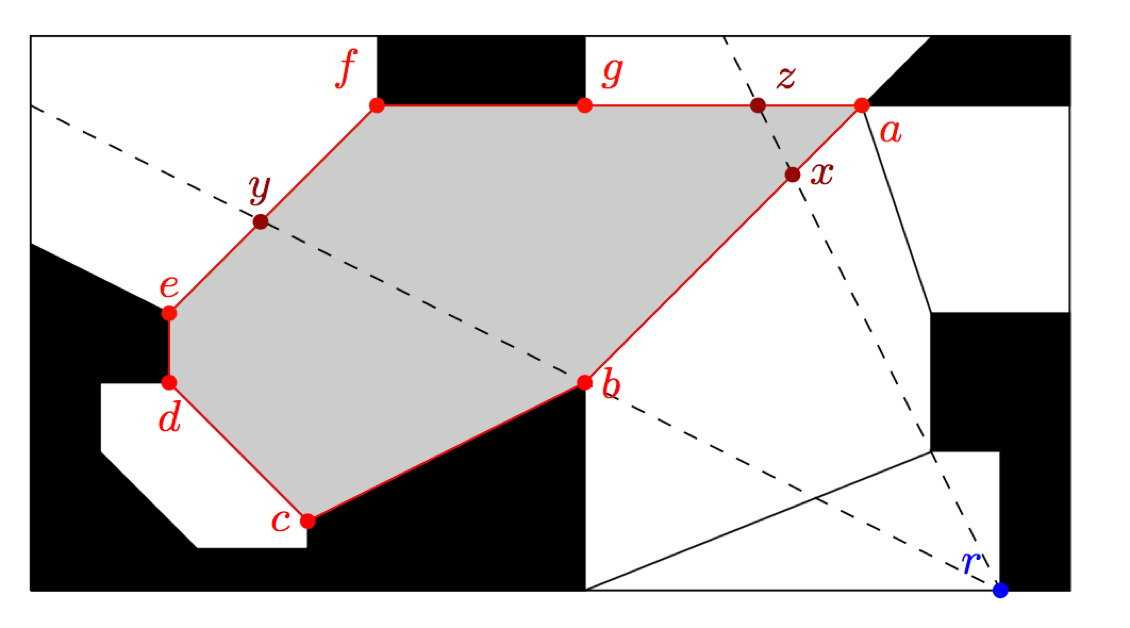
\includegraphics[width=.6\linewidth]{pic/suc.png}
    \caption{\small We expand the node $([e,c],q)$ which has
    $([c,g],q)$ and $[h, j], q$ as observable successors.
    In addition, the nodes $([e,f],e)$, $([f,j],e)$ are non-observable.
    All other potential successors can be safely pruned (more details in~\cite{cuicompromise}).}
    \label{suc}
  \end{figure}

\pagebreak
\item \textbf{Evaluation}: When prioritising nodes for expansion, \textit{Polyanya} makes use of an
  \textit{f-value} estimation function which bounds the length of the optimal path:
  from $q$, throught the current node (i.e. via some $p \in I$) and onto the target. There are
  three cases to consider which describe the relative positions of the target in relation to
  the current node. These are illustrated in Figure~\ref{ef}. The objective in each case is to
  choose the unique $p \in I$ that minimise the estimate. The three cases together are
  sufficient to guarantee that the estimator is admissible.

  \begin{figure}[htp]
    \centering
    \begin{tikzpicture}[line cap=round,line join=round,>=triangle 45,x=.7cm,y=.7cm]
\newcommand{\degre}{\ensuremath{^\circ}}
\definecolor{qqwuqq}{rgb}{0.,0.39215686274509803,0.}
\definecolor{ududff}{rgb}{0.30196078431372547,0.30196078431372547,1.}
\definecolor{ffqqqq}{rgb}{1.,0.,0.}
\definecolor{cqcqcq}{rgb}{0.7529411764705882,0.7529411764705882,0.7529411764705882}

%\draw [color=cqcqcq,, xstep=2.0cm,ystep=2.0cm] (-2.5,-1.5) grid (11.1,5.5);
\clip(-2.5,-1.5) rectangle (11.1,5.5);
\draw [thick,color=qqwuqq,fill=qqwuqq,fill opacity=0.10000000149011612] (5.882794718512914,1.3724017604956955) -- (6.1103929580172185,2.0551964790086092) -- (5.427598239504305,2.282794718512914) -- (5.2,1.6) -- cycle; 
\draw [thick,color=ffqqqq] (1.,3.)-- (10.,0.);
\draw [thick,dash pattern=on 1pt off 3pt,domain=-2.5:11.1] plot(\x,{(-42.--9.*\x)/3.});
\draw [thick] (-2.,0.)-- (1.,3.);
\draw [thick] (1.,3.)-- (0.,4.);
\draw [thick] (-2.,0.)-- (6.,4.);
\draw [thick] (4.4,-0.8)-- (2.8,2.4);
\begin{scriptsize}
\draw [fill=ffqqqq] (1.,3.) circle (2.5pt);
\draw[color=ffqqqq] (1.2251463573152723,3.6132615238618353) node {\large $a$};
\draw [fill=ffqqqq] (10.,0.) circle (2.5pt);
\draw[color=ffqqqq] (10.623297185327285,-0.2884978451684127) node {\large $b$};
\draw [fill=ududff] (-2.,0.) circle (2.5pt);
\draw[color=ududff] (-2.269472903642263,0.8989941367103583) node {\large $r$};
\draw [fill=ffqqqq] (0.,4.) circle (2.5pt);
\draw[color=ffqqqq] (-0.3864499038059212,5.190929442643631) node {\large $t_2$};
\draw [fill=ffqqqq] (6.,4.) circle (2.5pt);
\draw[color=ffqqqq] (5.347439951551588,5.021287730946663) node {\large $t_1$};
\draw[color=qqwuqq] (6.585824446939453,1.9507727492315556) node {\large $\alpha = 90\textrm{\degre}$};
\draw [fill=ffqqqq] (4.4,-0.8) circle (2.5pt);
\draw[color=ffqqqq] (3.413524438206156,-0.3393903586775029) node {\large $t_3$};
\end{scriptsize}
\end{tikzpicture}

    \caption{\small
    Polyanya $f$-value estimator. The current node is $(I, r)$ with $I = [a, b]$ and
    each of $t_1, t_2, t_3$ are possible target locations.
    \textbf{Case 1}: the target is $t_1$. In this case the point $p \in I$ with minimum
    $f$-value is at the intersection of the interval $I$ and the line $r \rightarrow t_1$.
    \textbf{Case 2}: the target is $t_2$. In this case the $p \in I$ with minimum $f$-value
    is one of two endpoints of $I$. 
    \textbf{Case 3}: the target is $t_3$. In this case the $p \in I$ with minimum $f$-value
    is obtained by first mirroring $t_3$ through $[a, b]$ and applying Case 1 or Case 2
    to the mirrored point (here, $t_1$). Notice that in this case, simply $r$ to $t_3$
    doesn't give us the \textit{h-value}, based on definition, it must reach the interval
    first.
    }
  \label{ef}
  \end{figure}
\end{itemize}

Similar to \textit{A*}, \textit{Polyanya} terminates when the target is expanded or when the
open list is empty. Extending it to multi-target OkNN is not a trivial problem, we will discuss
this in chapter~\ref{proposedalgo}.

\section{Other Obstacle Spatial Queries}\label{lrquery}
Obstacle spatial query processing is a broad research area, and many existing works are still
based on visibility graph, in this section, we review those works which can get benefit from
the OkNN in our research. 

\begin{itemize}

\item \textbf{Obstacle Range Query}(OR): given the query point $q$ and a range $r$,
  it returns all targets which obstacle distance to $q$ are less or equal to $r$ \cite{zhang2004spatial}. 
To solve this by OkNN, we can let $k$ be infinite and terminate the algorithm when current
obstacle distance large than $r$.

\item \textbf{Obstacle Reverse k-Nearest Neighbor}(ORkNN): it is proposed in
2011\cite{gao2011efficient} for $k=1$, and be generalized to $k>1$ in
2016\cite{gao2016reverse}. ORkNN given query point $q$ and $k$, return a set of targets which
regards $q$ as its OkNN: $\{t | q \in OkNN(t, k)\}$. The query processing has two stages:
(i) \textit{search stage}: explore search space to get a set of candidates; (ii) \textit{refine
stage}: calls OkNN for each candidate, remove a candidate if $q$ is not its OkNN.
The first stage needs to compute obstacle distance to prune search space, and the second stage 
can directly get benefit from the improvement of OkNN.

\item \textbf{Continuous Obstacle k-Nearest Neighbor}(COkNN): it's proposed in
  2009\cite{gao2009continuous}, similar to OkNN, but the query becomes a segment.
  The algorithm first generates a list of "split" points, and reduce the problem to finding the
    OkNN for these points. It also needs to compute obstacle distance to prune search space.

\end{itemize}

\section{Summary}
In this chapter, we've reviewed works that are related to our research.
We firstly introduced the background knowledge by discussing $\textit{A}^*$ and
\textit{Dijkstra}. 
Then we discussed existing works basically from three fields: Spatial Index, Spatial Query Processing and AI Pathfinding.
The major finding is that, in OkNN problem, existing VG based algorithms are hard to improve,
so we are motivated to look for a new framework, meanwhile,
the new work in AI Pathfinding field shows us a new direction.
